
	Si bien hasta ahora en la simulación se han utilizado datos de las mediciones en forma equiespaciada, en las aplicaciones prácticas muchas veces no se sabe en que momento se recibirá la próxima medición, o incluso, puede darse que recibamos información de distintos sensores con distinta frecuencia. El objetivo de este punto es ver como se comporta el filtro de Kalman ante la falta o perdida de datos en algunos instantes. Para poder simular esto disponemos de dos mecanismos distintos. La primera manera de simularlo es utilizando una matriz de salida $C_d$ dinámica que se modifique en funcion de los datos de los sensores disponibles en un determinado instante. La segunda variante es utilizar una matriz $C_d$ de tamaño fijo, e incertar ceros en lugar de las matrices identidades, cada vez que se pierde un dato o no se dispone de una medición de ese sensor. Dado a que disponer de memoria dinámica para la matriz $C_d$ es un poco mas costoso en los sistemas reales, se ha optado por la segunda alternativa.
	
	En la figura \ref{fig:ej7_1} puede verse lo que sucede si se pierden un 10 \% de las mediciones. Puede verse que en este caso el resultado no es severo. Por otro lado en la figura \ref{fig:ej7_2} se representa lo que sucede cuando se pierden un 90 \% de las mediciones. Cuando el filtro deja de recibir información de los sensores, continuará estimando con la dinámica del sistema. En el segundo caso se observa que cada vez que ocurren largos lapsos en los que no recibe mediciones, el error de estimación crece cada vez mas, hasta que se recibe una nueva medición que lo vuelve a colocar en la trayectoria.
	
	\begin{figure}[H]
		\centering
		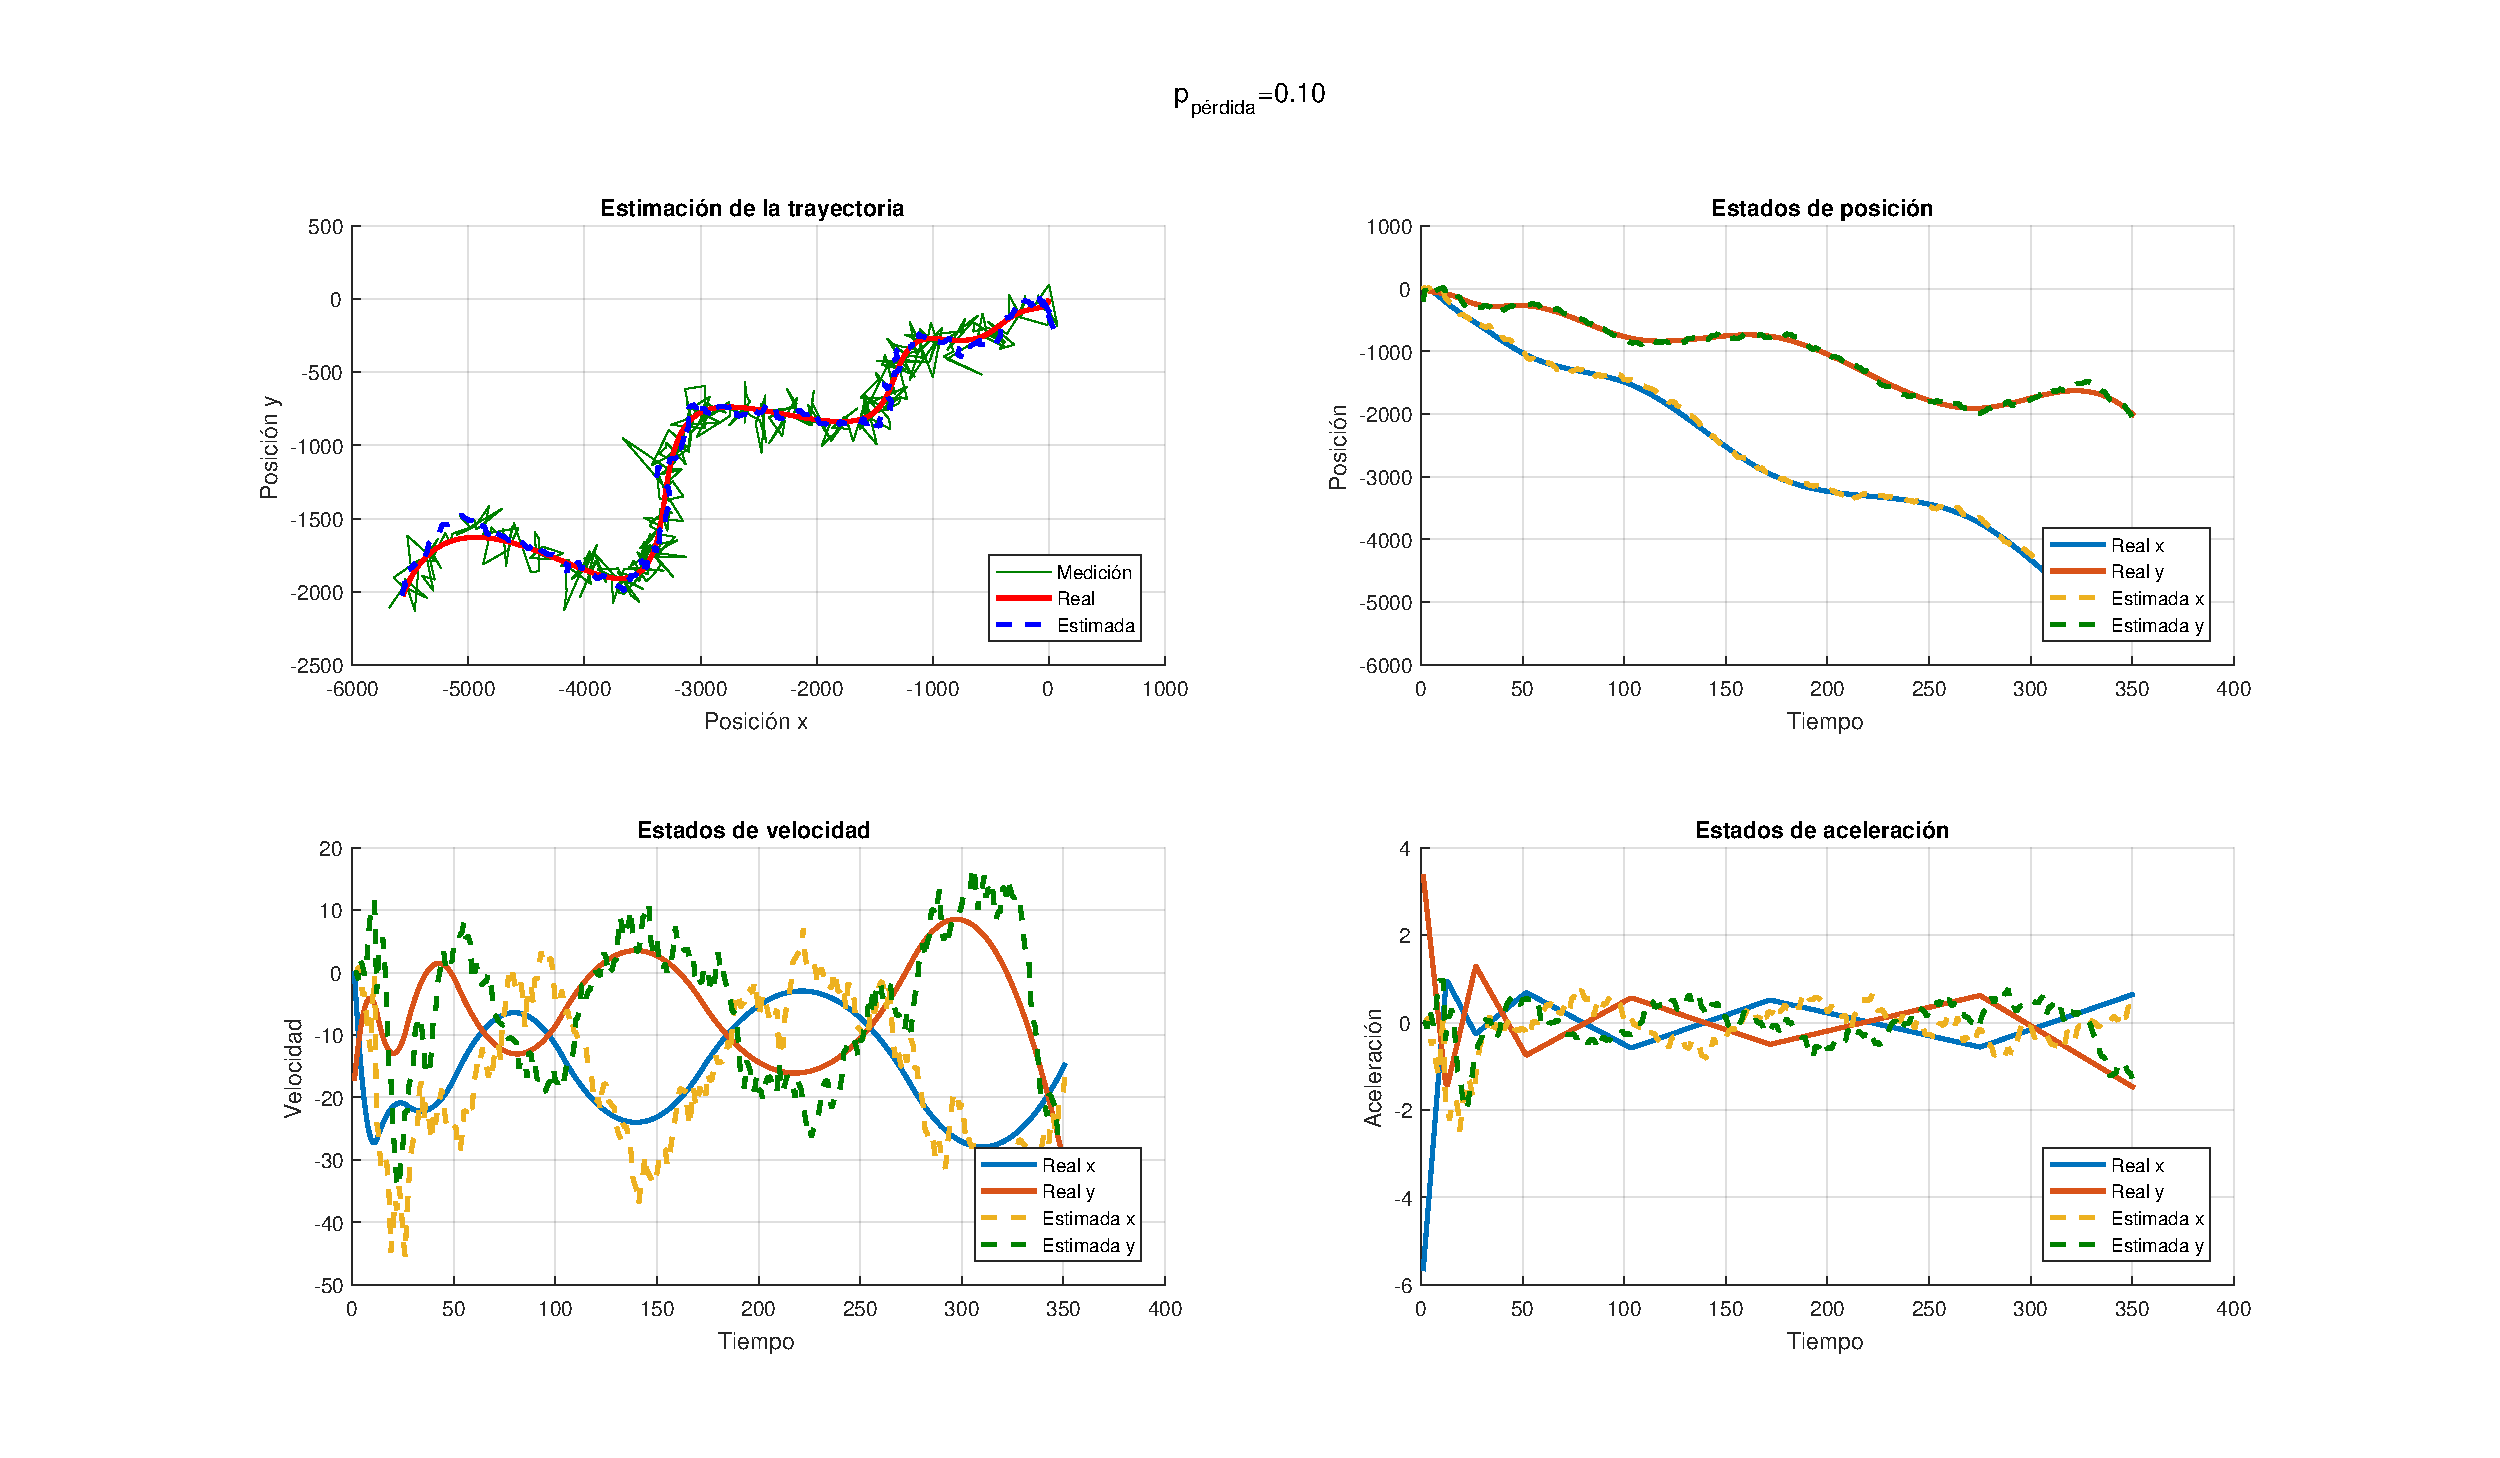
\includegraphics[width=1.0\textwidth,keepaspectratio]{Figuras/graf_ej7_1.pdf}
		\caption{Estimación De Trayectoria - Perdida Del 10 \%}
		\label{fig:ej7_1}
	\end{figure}
	
	\begin{figure}[H]
		\centering
		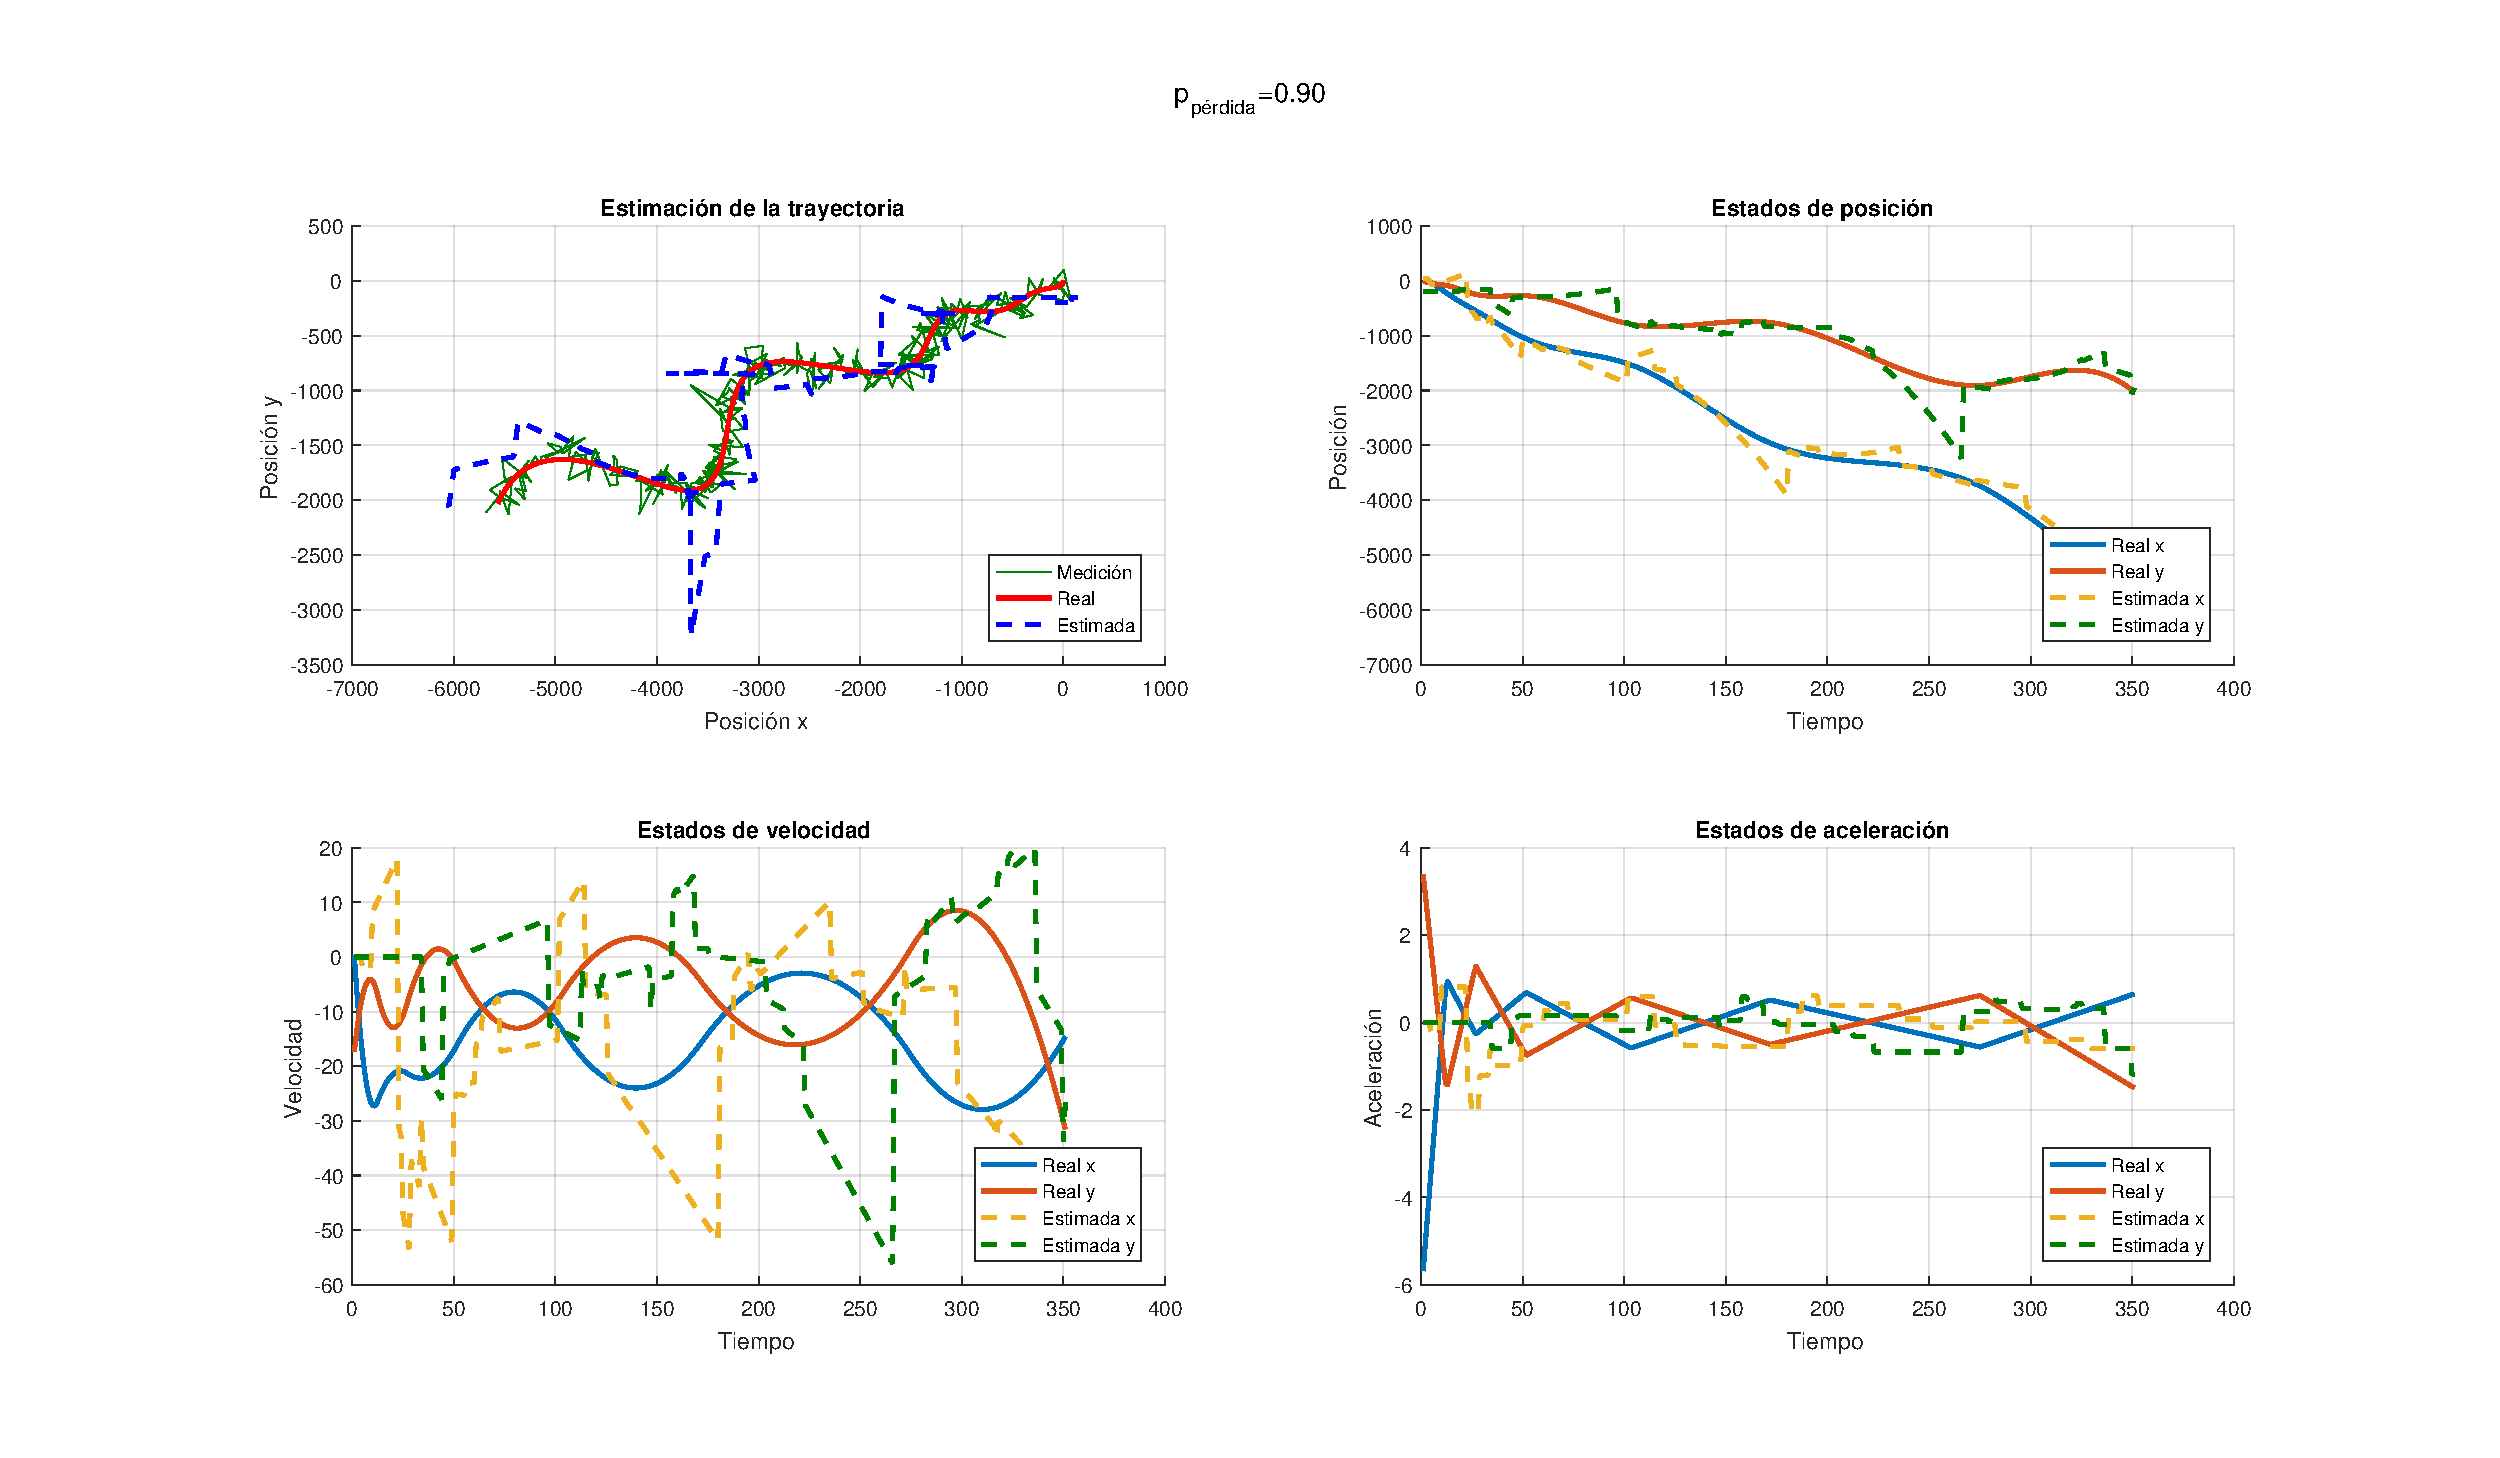
\includegraphics[width=1.0\textwidth,keepaspectratio]{Figuras/graf_ej7_2.pdf}
		\caption{Estimación De Trayectoria - Perdida Del 90 \%}
		\label{fig:ej7_2}
	\end{figure}
	
	En las figuras \ref{fig:ej7_1_inov} y \ref{fig:ej7_1_inov} podemos ver la autocorrelación de las innovaciones. Cuanto mas se parezcan a ruido blanco, significa que mejor es la estimación, es decir, que todo lo que no puede predecir el filtro, corresponde a ruido blanco. Puede verse que cuatas menos mediciones se tiene, menos se da esta propiedad.
	
	\begin{figure}[H]
		\centering
		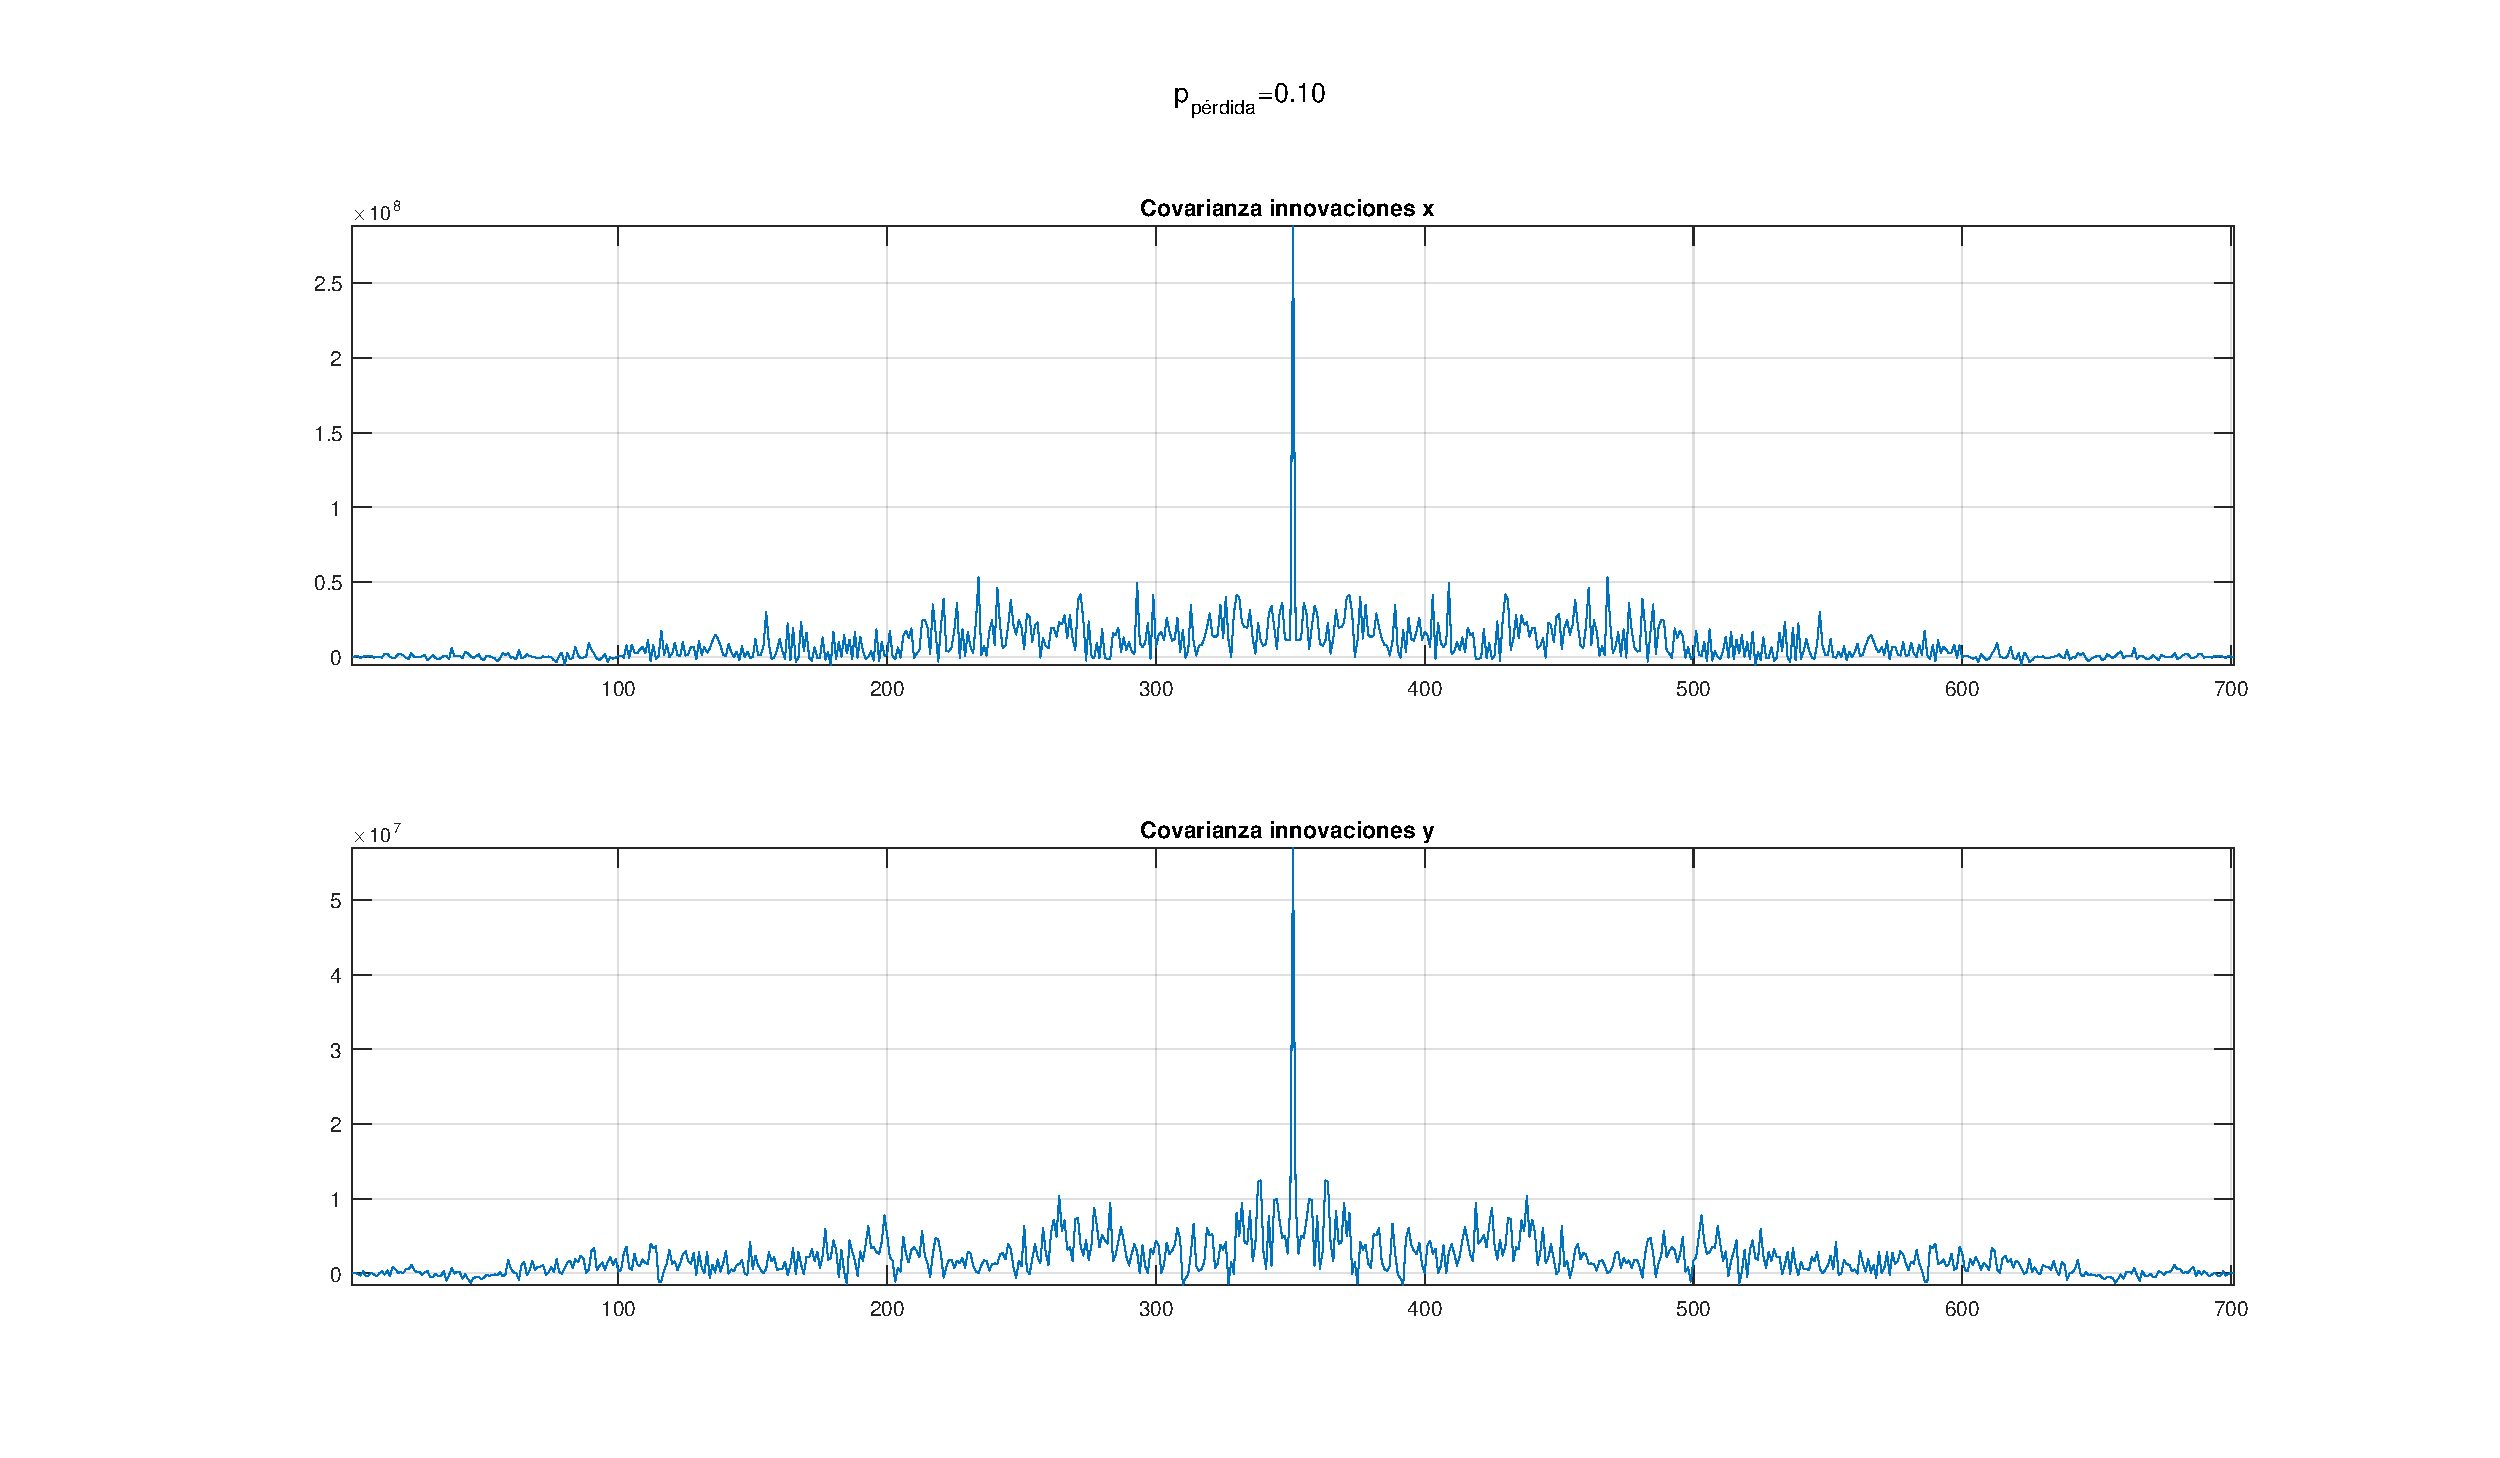
\includegraphics[width=1.0\textwidth,keepaspectratio]{Figuras/covinn_ej7_1.pdf}
		\caption{Autocorrelación De Innovaciones - Perdida Del 10 \%}
		\label{fig:ej7_1_inov}
	\end{figure}
	
	\begin{figure}[H]
		\centering
		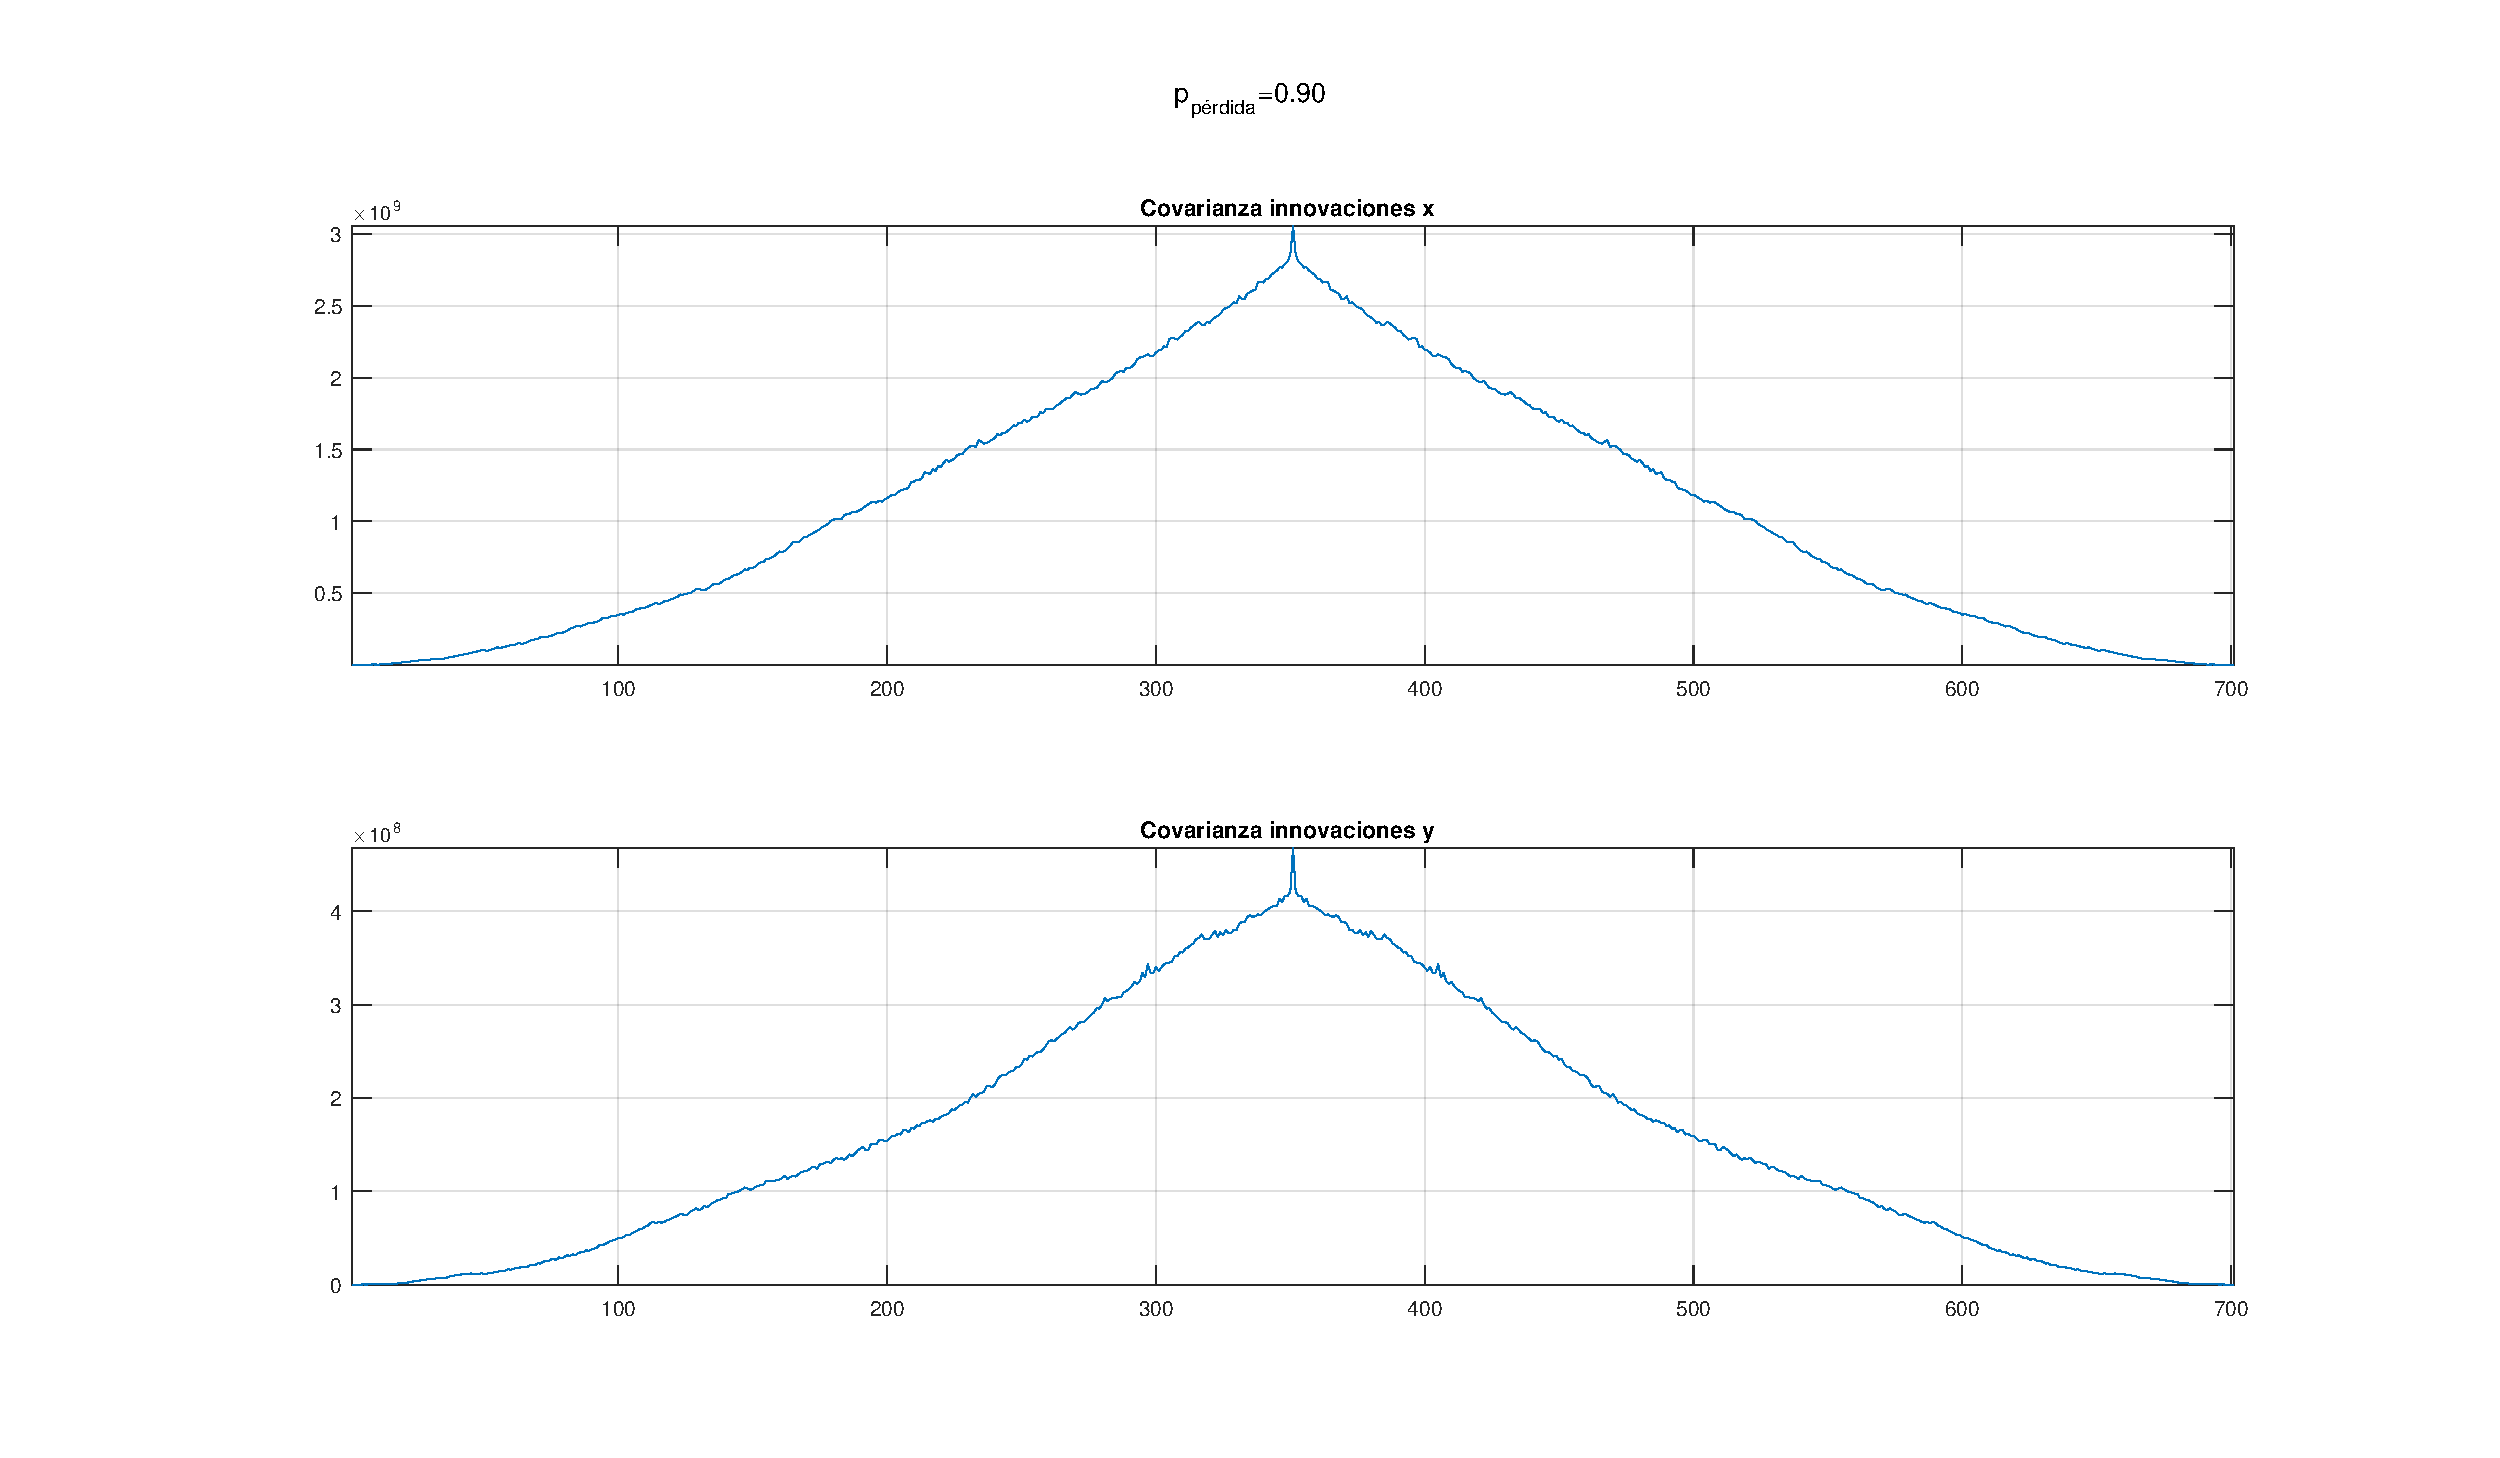
\includegraphics[width=1.0\textwidth,keepaspectratio]{Figuras/covinn_ej7_2.pdf}
		\caption{Autocorrelación De Innovaciones - Perdida Del 90 \%}
		\label{fig:ej7_1_inov}
	\end{figure}
